% ============================================================
% 第12章：极限存在判别法——单调有界、夹逼、柯西
% ============================================================

\chapter{极限存在判别法——单调有界与夹逼定理}

\begin{applicationbox}
\textbf{学完本章你能做什么？}
\begin{enumerate}
  \item 用\textbf{单调有界原理}判断数列收敛——这是数学分析中最常用的方法
  \item 用\textbf{夹逼定理}（迫敛性）求极限——把复杂数列夹在两个简单数列之间
  \item 了解\textbf{柯西收敛准则}——不依赖极限值也能判断收敛
\end{enumerate}
\end{applicationbox}


% ============================================================
\section{从第11章来——如何判断极限存在？}
% ============================================================

第11章我们学了极限的 ε-N 定义——但用定义证明收敛，需要\textbf{先知道极限值}。

如果不知道极限值呢？比如数列 \(a_n = (1 + \frac{1}{n})^n\)——它有极限吗？极限是多少？

这就需要用到本章的两个强大工具：
\begin{itemize}
  \item \textbf{单调有界原理}：如果数列单调且有界，则一定收敛
  \item \textbf{夹逼定理}：如果两个数列收敛到同一个数，中间那个也收敛
\end{itemize}


% ============================================================
\section{单调有界原理}
% ============================================================

\begin{theorembox}[单调有界原理]
如果数列 \(\{a_n\}\) 是\textbf{单调递增}且\textbf{有上界}的，那么它一定收敛。

同样，如果数列是\textbf{单调递减}且\textbf{有下界}的，那么它一定收敛。
\end{theorembox}

\begin{examplebox}[1——单调有界的直观]
\begin{center}
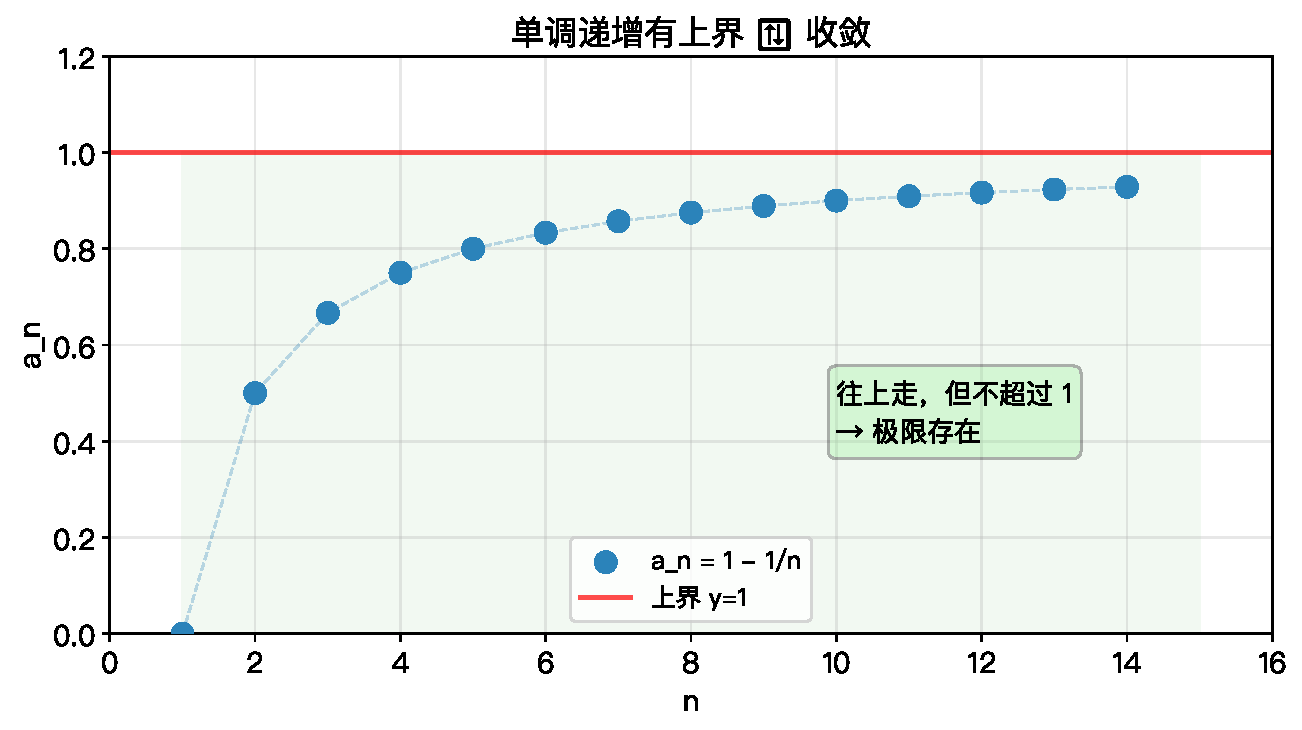
\includegraphics[width=0.85\textwidth]{figures/ch12_monotone_bounded.pdf}
\end{center}

数列 \(a_n = 1 - \frac{1}{n}\)：
\begin{itemize}
  \item \textbf{单调递增}：\(a_1=0, a_2=0.5, a_3\approx0.667, a_4=0.75, \ldots\)——一直往上走
  \item \textbf{有上界}：永远不超过 1（因为 \(\frac{1}{n} > 0\)，所以 \(1 - \frac{1}{n} < 1\)）
  \item \(\rightarrow\) \textbf{收敛}，极限为 1
\end{itemize}

\textbf{为什么单调有界一定收敛？}
从直观看：单调递增有上界，数列一直往上走但不能突破上界，所以它只能"挤"在某个数附近——这个数就是极限。
\end{examplebox}

\begin{examplebox}[2——求极限的重要方法]
用单调有界原理求极限的\textbf{标准步骤}：

\begin{enumerate}
  \item 证明数列\textbf{单调}（常用 \(a_{n+1} - a_n \ge 0\) 或 \(\frac{a_{n+1}}{a_n} \ge 1\)）
  \item 证明数列\textbf{有界}（找到上界或下界）
  \item 由单调有界原理 \(\Rightarrow\) 极限存在（设为 \(L\)）
  \item 在递推式两边取极限，解出 \(L\)
\end{enumerate}
\end{examplebox}

\begin{examplebox}[3——用单调有界求极限]
已知 \(a_1 = 2\)，\(a_{n+1} = \frac{1}{2}\left(a_n + \frac{2}{a_n}\right)\)。

\textbf{第1步：证有下界}
\[
a_{n+1} = \frac{1}{2}\left(a_n + \frac{2}{a_n}\right) \ge \frac{1}{2} \cdot 2\sqrt{a_n \cdot \frac{2}{a_n}} = \sqrt{2}
\]
（用基本不等式：\(x + \frac{2}{x} \ge 2\sqrt{2}\)）

所以 \(a_n \ge \sqrt{2}\) 对所有 \(n\) 成立。

\textbf{第2步：证单调递减}
\[
a_{n+1} - a_n = \frac{1}{2}\left(a_n + \frac{2}{a_n}\right) - a_n = \frac{1}{2}\left(\frac{2}{a_n} - a_n\right) = \frac{2 - a_n^2}{2a_n} \le 0
\]
（因为 \(a_n \ge \sqrt{2}\)，所以 \(a_n^2 \ge 2\)，分子 \(\le 0\)）

所以 \(a_{n+1} \le a_n\)，单调递减。

\textbf{第3步：极限存在}
单调递减有下界 \(\Rightarrow\) 极限存在，设 \(\lim a_n = L\)。

\textbf{第4步：求极限}
在递推式两边取极限：
\[
L = \frac{1}{2}\left(L + \frac{2}{L}\right) \;\Longrightarrow\; 2L = L + \frac{2}{L} \;\Longrightarrow\; L = \frac{2}{L} \;\Longrightarrow\; L^2 = 2
\]
所以 \(L = \sqrt{2}\)（因为 \(a_n > 0\)，舍去负值）。

\textbf{结论：} \(\displaystyle \lim_{n\to\infty} a_n = \sqrt{2}\)。
\end{examplebox}


% ============================================================
\section{夹逼定理（迫敛性）}
% ============================================================

\begin{theorembox}[夹逼定理]
如果存在 \(N\) 使得 \(n > N\) 时
\[
b_n \le a_n \le c_n
\]
且 \(\displaystyle \lim_{n\to\infty} b_n = \lim_{n\to\infty} c_n = L\)，
则 \(\displaystyle \lim_{n\to\infty} a_n = L\)。
\end{theorembox}

\textbf{直观理解：} 三个人挤在一条巷子里，两边的人都出去了，中间那个人也只能从那个口出去。

\begin{examplebox}[4——夹逼定理的几何意义]
\begin{center}
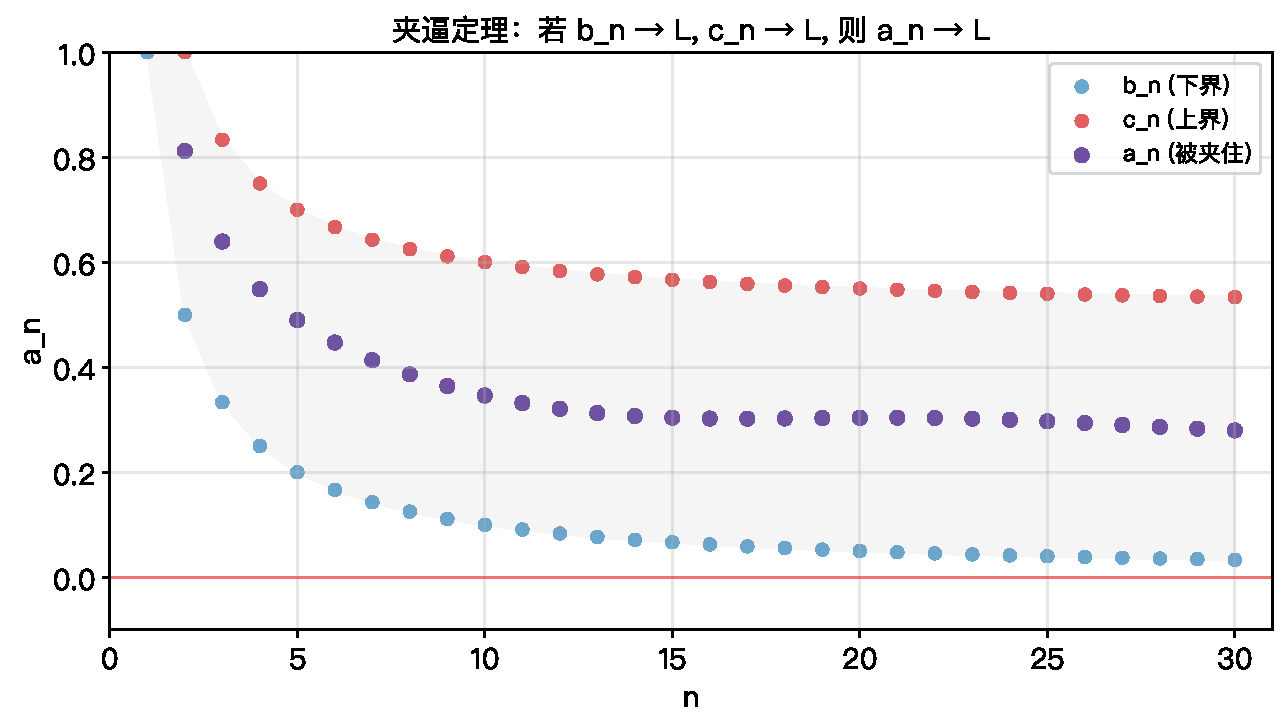
\includegraphics[width=0.85\textwidth]{figures/ch12_squeeze_theorem.pdf}
\end{center}

灰色区域是 \(b_n\) 和 \(c_n\) 夹出的范围，\(a_n\) 被限制在其中。
当 \(b_n\) 和 \(c_n\) 都趋近于同一个数时，\(a_n\) 也只能趋近于那个数。
\end{examplebox}

\begin{examplebox}[5——用夹逼定理求极限]
求 \(\displaystyle \lim_{n\to\infty} \frac{\sin n}{n}\)。

因为 \(|\sin n| \le 1\)，所以：
\[
-\frac{1}{n} \le \frac{\sin n}{n} \le \frac{1}{n}
\]

而 \(\displaystyle \lim_{n\to\infty} \left(-\frac{1}{n}\right) = 0\)，\(\displaystyle \lim_{n\to\infty} \frac{1}{n} = 0\)。

由夹逼定理：\(\displaystyle \lim_{n\to\infty} \frac{\sin n}{n} = 0\)。
\end{examplebox}

\begin{examplebox}[6——另一个例子]
求 \(\displaystyle \lim_{n\to\infty} \frac{n!}{n^n}\)。

\[
0 < \frac{n!}{n^n} = \frac{1 \cdot 2 \cdot 3 \cdots n}{n \cdot n \cdot n \cdots n} \le \frac{1}{n}
\]

而 \(0 \to 0\)，\(\frac{1}{n} \to 0\)，由夹逼定理：
\[
\lim_{n\to\infty} \frac{n!}{n^n} = 0
\]
\end{examplebox}


% ============================================================
\section{两个重要极限}
% ============================================================

\begin{theorembox}[两个重要极限]
\[
(1)\; \lim_{n\to\infty} \left(1 + \frac{1}{n}\right)^n = e
\]
\[
(2)\; \lim_{n\to\infty} \sqrt[n]{n} = 1
\]
\end{theorembox}

\begin{examplebox}[7——第一个重要极限：自然常数 \(e\)]
数列 \(a_n = \left(1 + \frac{1}{n}\right)^n\)：
\[
a_1 = 2,\; a_2 = (1.5)^2 = 2.25,\; a_3 \approx 2.37,\; a_{10} \approx 2.594
\]
\[
a_{100} \approx 2.705,\; a_{1000} \approx 2.717,\; a_{10000} \approx 2.718
\]

这个数列\textbf{单调递增且有上界}（可以证明上界为 3），
因此收敛——它的极限就是 \(e \approx 2.71828\)。

这是自然常数 \(e\) 的\textbf{定义}之一。
\end{examplebox}

\begin{examplebox}[8——第二个重要极限]
证明 \(\sqrt[n]{n} \to 1\)：

令 \(\sqrt[n]{n} = 1 + x_n\)（\(x_n > 0\)），则：
\[
n = (1 + x_n)^n \ge 1 + \frac{n(n-1)}{2}x_n^2 \quad (\text{二项式展开到第三项})
\]
\[
\Rightarrow x_n^2 \le \frac{2(n-1)}{n(n-1)} = \frac{2}{n-1}
\]
\[
\Rightarrow 0 < x_n \le \sqrt{\frac{2}{n-1}} \to 0
\]

由夹逼定理，\(x_n \to 0\)，所以 \(\sqrt[n]{n} = 1 + x_n \to 1\)。
\end{examplebox}


% ============================================================
\section{柯西收敛准则（了解）}
% ============================================================

\begin{theorembox}[柯西收敛准则]
数列 \(\{a_n\}\) 收敛的\textbf{充要条件}是：
对任意 \(\varepsilon > 0\)，存在 \(N\)，使得 \(m, n > N\) 时
\[
|a_m - a_n| < \varepsilon
\]
\end{theorembox}

\textbf{含义：} 收敛数列的项越到后面"挤得越紧"——任意两项的差最终可以任意小。

柯西准则的\textbf{优点}：不需要知道极限值就能判断收敛。\\
\textbf{缺点}：使用起来比单调有界和夹逼更复杂。


% ============================================================
\section{本章小结}
% ============================================================

\begin{progressbox}
\textbf{单调有界原理}：单调递增有上界（或递减有下界）⇒ 收敛

\textbf{证明步骤}：证单调 $\to$ 证有界 $\to$ 极限存在 $\to$ 在递推式两边取极限求值

\textbf{夹逼定理}：\(b_n \le a_n \le c_n\)，且 \(b_n, c_n \to L\) ⇒ \(a_n \to L\)

\textbf{两个重要极限}：
\[
\lim_{n\to\infty} \left(1 + \frac{1}{n}\right)^n = e,\quad
\lim_{n\to\infty} \sqrt[n]{n} = 1
\]

\textbf{柯西准则}：\(m,n\) 足够大时 \(|a_m - a_n| < \varepsilon\) ⇔ 收敛
\end{progressbox}

\subsection*{通往第二编——函数极限与连续}


% ============================================================
% 习题
% ============================================================
\section{习题}

% ===== 送分 =====

\begin{exercise}[0]
判断正误：单调递增的数列一定收敛。
\end{exercise}

\begin{exercise}[0]
判断正误：有上界的数列一定收敛。
\end{exercise}

\begin{exercise}[0]
数列 \(a_n = 1 - \frac{1}{n}\) 是否单调？是否有上界？
\end{exercise}

\begin{exercise}[0]
夹逼定理中，如果 \(b_n \le a_n \le c_n\) 且 \(b_n \to 2\)，\(c_n \to 2\)，则 \(a_n \to\) \_\_\_\_。
\end{exercise}

% ===== 简单 =====

\begin{exercise}[1]
证明数列 \(a_n = \frac{n}{n+1}\) 单调递增且有上界，并求极限。
\end{exercise}

\begin{exercise}[1]
用夹逼定理求 \(\displaystyle \lim_{n\to\infty} \frac{\cos n}{n}\)。
\end{exercise}

\begin{exercise}[1]
判断：数列 \(a_n = (-1)^n\) 是否单调？是否有界？是否收敛？
\end{exercise}

\begin{exercise}[1]
已知 \(a_n = 2 - \frac{1}{n}\)，证明它单调递增且有上界，极限是多少？
\end{exercise}

% ===== 基础 =====

\begin{exercise}[2]
用单调有界原理证明数列 \(a_n = \frac{1}{2^n}\) 收敛，并求极限。
\end{exercise}

\begin{exercise}[2]
用夹逼定理求 \(\displaystyle \lim_{n\to\infty} \frac{n + \sin n}{2n - \cos n}\)。
（提示：放大到 \(\frac{n+1}{2n-1}\)，缩小到 \(\frac{n-1}{2n+1}\)）
\end{exercise}

\begin{exercise}[2]
求极限 \(\displaystyle \lim_{n\to\infty} \left(1 + \frac{1}{n}\right)^n\)，这个极限等于什么常数？
\end{exercise}

\begin{exercise}[2]
求证：数列 \(a_n = \frac{1}{2} \cdot \frac{3}{4} \cdot \frac{5}{6} \cdots \frac{2n-1}{2n}\) 单调递减且有下界。
\end{exercise}

% ===== 普通 =====

\begin{exercise}[3]
已知 \(a_1 = 1\)，\(a_{n+1} = \sqrt{2a_n}\)。
\begin{enumerate}
  \item[(1)] 写出前 4 项
  \item[(2)] 证明 \(\{a_n\}\) 单调递增且有上界
  \item[(3)] 求极限
\end{enumerate}
\end{exercise}

\begin{exercise}[3]
用夹逼定理求 \(\displaystyle \lim_{n\to\infty} \frac{\ln n}{n}\)。
（提示：\(0 < \frac{\ln n}{n} < \frac{1}{\sqrt{n}}\) 当 \(n\) 足够大时）
\end{exercise}

\begin{exercise}[3]
已知 \(a_n = \frac{n!}{2^n}\)。证明 \(a_n \to \infty\)（发散）。
（提示：\(n \ge 4\) 时 \(\frac{a_{n+1}}{a_n} = \frac{n+1}{2} > 1\)）
\end{exercise}

\begin{exercise}[3]
求极限 \(\displaystyle \lim_{n\to\infty} \frac{2^n}{n!}\)。
（提示：\(n \ge 4\) 时 \(\frac{2^n}{n!} \le \frac{2}{n}\)，再用夹逼定理）
\end{exercise}

\begin{exercise}[3]
证明数列 \(a_n = \left(1 + \frac{1}{n}\right)^{n+1}\) 单调递减。
（提示：可以证明 \(\frac{a_{n+1}}{a_n} \le 1\)）
\end{exercise}

% ===== 中等 =====

\begin{exercise}[4]
已知 \(a_1 = \sqrt{2}\)，\(a_{n+1} = \sqrt{2 + a_n}\)。
\begin{enumerate}
  \item[(1)] 证明 \(a_n < 2\) 对所有 \(n\) 成立
  \item[(2)] 证明 \(\{a_n\}\) 单调递增
  \item[(3)] 求极限
\end{enumerate}
\end{exercise}

\begin{exercise}[4]
用夹逼定理求 \(\displaystyle \lim_{n\to\infty} \left(\frac{1}{\sqrt{n^2+1}} + \frac{1}{\sqrt{n^2+2}} + \cdots + \frac{1}{\sqrt{n^2+n}}\right)\)。
（提示：\(n\) 项，每项介于 \(\frac{1}{\sqrt{n^2+n}}\) 和 \(\frac{1}{\sqrt{n^2}}\) 之间）
\end{exercise}

\begin{exercise}[4]
已知 \(a_1 = 1\)，\(a_{n+1} = \frac{a_n}{2} + \frac{1}{a_n}\)。
\begin{enumerate}
  \item[(1)] 证明 \(a_n^2 \ge 2\)
  \item[(2)] 证明数列单调递减
  \item[(3)] 求极限
\end{enumerate}
\end{exercise}

\begin{exercise}[4]
求 \(\displaystyle \lim_{n\to\infty} \frac{1}{n^2} \left( \frac{1}{1^2} + \frac{1}{2^2} + \cdots + \frac{1}{n^2} \right)\)。
\end{exercise}

\begin{exercise}[4]
证明：若 \(0 < a < 1\)，则 \(a^n \to 0\)（用夹逼定理）。
\end{exercise}

% ===== 进阶 =====

\begin{exercise}[5]
已知 \(a_1 = 3\)，\(a_{n+1} = \frac{1}{2}\left(a_n + \frac{9}{a_n}\right)\)。
\begin{enumerate}
  \item[(1)] 证明 \(a_n \ge 3\)
  \item[(2)] 证明单调递减
  \item[(3)] 求极限
\end{enumerate}
\end{exercise}

\begin{exercise}[5]
用单调有界原理证明数列 \(a_n = \frac{1}{n+1} + \frac{1}{n+2} + \cdots + \frac{1}{2n}\) 收敛。
（提示：先证 \(a_{n+1} - a_n = \frac{1}{2n+1} - \frac{1}{2n+2} > 0\)，再证 \(a_n < 1\)）
\end{exercise}

\begin{exercise}[5]
求 \(\displaystyle \lim_{n\to\infty} \sqrt[n]{n^2 + 1}\)。
（提示：\(\sqrt[n]{n^2} \le \sqrt[n]{n^2+1} \le \sqrt[n]{2n^2}\)，且 \(\sqrt[n]{n} \to 1\)）
\end{exercise}

\begin{exercise}[5]
已知 \(0 < a_1 < 1\)，\(a_{n+1} = a_n(1 - a_n)\)。
\begin{enumerate}
  \item[(1)] 证明 \(0 < a_n < 1\) 且单调递减
  \item[(2)] 求极限
\end{enumerate}
\end{exercise}

% ===== 拔高 =====

\begin{exercise}[6]
已知 \(a_1 = 1\)，\(a_{n+1} = 1 + \frac{1}{a_n}\)。
\begin{enumerate}
  \item[(1)] 写出前 6 项，观察奇偶子列的规律
  \item[(2)] 证明 \(\{a_{2k}\}\) 和 \(\{a_{2k+1}\}\) 分别单调且收敛
  \item[(3)] 它们的极限相等吗？如果相等，求极限。
\end{enumerate}
（这个数列的极限是黄金分割比 \(\frac{1+\sqrt{5}}{2}\)——斐波那契数列的相邻项之比）
\end{exercise}

\begin{exercise}[6]
用夹逼定理证明 \(\displaystyle \lim_{n\to\infty} \frac{n}{\sqrt[n]{n!}} = e\)。
（提示：利用 \(n^n e^{-n} < n! < n^{n+1} e^{-n+1}\)，这是斯特林公式的粗略形式）
\end{exercise}

\begin{exercise}[6]
已知 \(a_1 > 0\)，\(a_{n+1} = \frac{a_n^2 + 1}{2a_n}\)。
\begin{enumerate}
  \item[(1)] 证明 \(a_n \ge 1\)
  \item[(2)] 证明单调递减
  \item[(3)] 求极限
\end{enumerate}
\end{exercise}

% ===== 极难 =====

\begin{exercise}[7]
设 \(a_1 = 1\)，\(a_{n+1} = \frac{3a_n + 2}{a_n + 2}\)。
\begin{enumerate}
  \item[(1)] 证明 \(a_n > 0\) 且有上界 2
  \item[(2)] 判断单调性并证明
  \item[(3)] 求极限
  \item[(4)] 若 \(b_n = \frac{a_n - 2}{a_n + 1}\)，证明 \(\{b_n\}\) 是等比数列
\end{enumerate}

\textbf{说明：} 这道题综合了单调有界原理和构造等比数列的技巧。
第(4)问的构造法——通过线性变换将递推式化为等比数列——是数学分析中处理递推数列的重要方法。
\end{exercise}



\textbf{第一编到此结束！} 你完成了数列极限的全部 4 章——
从数列基础到 ε-N 定义，再到单调有界和夹逼。

\textbf{第二编}我们将进入\textbf{函数极限与连续}——
把极限的思想从离散的数列扩展到连续的函数。
这是通向导数的大门。
